\lecture{Reti di fluidi}{06~-~10~-~2026}
%
\section{Fluidi}
Si tratta di fluidi caratterizzati dal fatto che in determinate condizioni di temperatura e pressione, hanno un
volume proprio, ma assumono la forma del contenitore all'interno del quale si trovano.
Il principale fluido che consideriamo è l'acqua.
%
\section{Fluidostatica}

\subsection{Densità}
Un importante proprietà dei fluidi è la \textbf{densità}, definita dal rapporto tra la massa del fluido e il volume occupato nelle condizioni in cui si trova:
\begin{formula}[Densità]\label{th:densita}
    \[
        \rho = \frac{M}{V} \ (\si{kg/m^{3}})
    \]
\end{formula}
Nel caso dei liquidi la densità varia in funzione di \emph{temperatura} e \emph{pressione}, ma in molte applicazioni pratiche
(specialmente quando le variazioni di temperatura non sono elevate) si può assumere che la densità sia costante.
\begin{example}
    Considerando l'acqua alla pressione atmosferica, possiamo trovare una densità di 1000 kg/m3 alla temperatura di 4°C e di circa 960 kg/m3 quando la temperatura si avvicina a 100 °C.

    La variazione di densità è quasi irrisorio, per cui possiamo considerare la densità dell'acqua costante.
\end{example}
%
\subsection{Viscosità}
Si consideri un liquido inserito all'interno di un contenitore molto esteso, tale da avere una altezza $ h $ dal fondo del contenitore ($ AB $). Per mettere in moto la superficie libera del liquido ($ A'B' $) in modo che raggiunga una velocità $ v $, è necessario applicare una certa forza $ f $.

La forza da applicare per unità di superficie del liquido $ \frac{F}{A} $ dipende dalla velocità e dall'altezza del liquido,
secondo la seguente relazione
\begin{formula}[Viscosità]
    \[
        \frac{F}{A}= \mu \frac{v}{h} \ (\si{Pa \cdot s})
    \]
\end{formula}
Nella quale $ \mu $ (mu) è una proprietà dei fluidi chiamata viscosità dinamica e si misura in $ \si{Pa \cdot s} $; la viscosità dipende dalle condizioni in cui si trova il fluido e diminuisce all'aumentare della temperatura. Per i liquidi la viscosità dipende scarsamente dalla pressione, se non per valori molto elevati di quest'ultima.
Vedi figura \ref{fig:viscosita}.

\begin{figure}
    \centering
    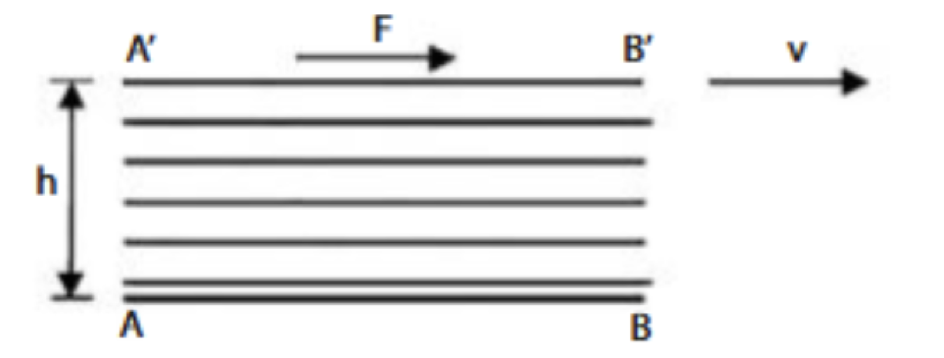
\includegraphics[width=0.5\linewidth]{assets/image.png}
    \caption{Viscosità}\label{fig:viscosita}
\end{figure}

%
\subsection{Pressione}

Si consideri un liquido fermo all'interno di un contenitore: la pressione sulla superficie (pelo) del liquido è la pressione atmosferica $ \si{p_{a}} $, la pressione all'interno aumenta all'aumentare della distanza dalla superficie secondo questa relazione:
\begin{formula}[Pressione]\label{th:pressione}
    \[
        p = p_{a} + \rho \cdot g \cdot h \ (\si{Pa})
    \]
    in cui $ p_{a} $ è la pressione atmosferica, $ g $ è l'accelerazione di gravità $ 9.81 \si{m/s^2} $, $ h $ è la distanza dalla superficie libera del liquido e $ \rho $ è la densità del liquido.
\end{formula}
Vedi figura \ref{fig:pressione}.
\begin{figure}
    \centering
    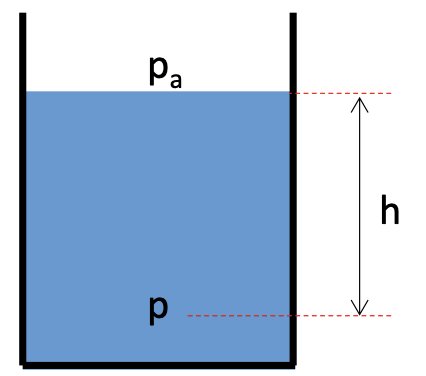
\includegraphics[width=0.4\linewidth]{assets/pressione.png}
    \caption{Pressione in un liquido statico}\label{fig:pressione}
\end{figure}

%
\section{Fluidodinamica}
%
\subsection{Portata in massa}
La portata in massa $ \dot{m} $ è definita come la massa nell'unità di tempo che passa attraverso una sezione aperta.
\begin{formula}[Portata in massa]
    Considerando un condotto di sezione $ A $ che trasporta acqua, la portata in massa è definita come:
    \[
        \dot{m} = \rho \cdot A \cdot v \ (\si{kg/s})
    \]
    in cui $ v $ è la velocità perpendicolare alla sezione $ A $ e $ \rho $ è la densità del fluido.
\end{formula}
\begin{figure}
    \centering
    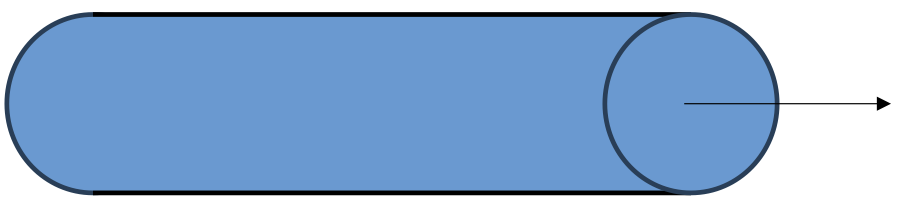
\includegraphics[width=0.8\linewidth]{assets/sezionea.png}
    \caption{Condotto di sezione $ A $}\label{fig:sezione}
\end{figure}\clearpage

La portata in massa si \emphgreen{conserva}.

In un condotto nel quale si ha un solo ingresso e una sola uscita, la portata in massa all'ingresso è uguale alla portata in massa all'uscita.
\[
    \dot{m}_{1} = \dot{m}_{2}
\]
Vedi figura \ref{fig:condotto2}.

\begin{figure}[h]
    \centering
    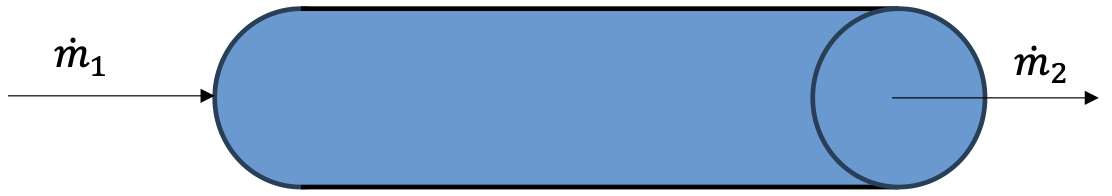
\includegraphics[width=0.8\linewidth]{assets/condotto2.png}
    \caption{La portata in massa $ \dot{m} $ si conserva}\label{fig:condotto2}
\end{figure}

Se si considera un condotto con più di due sezioni aperte (un miscelatore, un separatore di portata) la portata in ingresso è uguale alla somma delle portate in uscita.

\[
    \dot{m}_{1} = \dot{m}_{2} + \dot{m}_{3}
\]
Vedi figura \ref{fig:piuingressi}.
\begin{figure}[h]
    \centering
    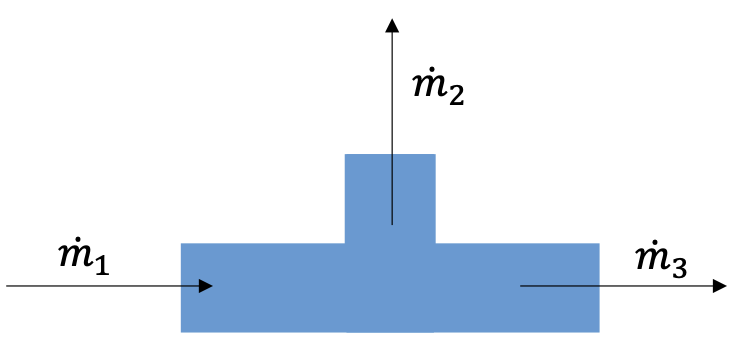
\includegraphics[width=0.8\linewidth]{assets/piuingressi.png}
    \caption{Componente con più sezioni aperte}\label{fig:piuingressi}
\end{figure}

\subsection{Regimi di moto dei fluidi}
Un fluido può assumere diversi regimi di moto: questi regimi sono legati al valore assunto dal numero di Reynolds $ R_{e} $.

\begin{description}
    \item [Laminare] Il moto è laminare quando il numero di Reynolds $ R_{e} < 2100 $
    \item [Transizione] Il moto è in transizione quando $ 2100 < R_{e} < 4300 $
    \item [Turbolento] Il moto è turbolento quando $ R_{e} > 4300 $
\end{description}

Il regime di moto determina l'attrito nel condotto e, di conseguenza, l'energia richiesta a pompe (nel caso di fluidi) o ventilatori (nel caso di gas) per ottenere un movimento.

%
\subsubsection{Numero di Reynolds}
\begin{formula}[Numero di Reynolds]
    L'espressione per un condotto cilindrico è:
    \[
        R_{e} = \frac{\rho \cdot v \cdot D}{\mu}
    \]
    in cui $ D $ è il diametro del condotto, $ \rho $ è la densità del fluido, $ v $ è la velocità del fluido e $ \mu $ è la viscosità del fluido.
\end{formula}

%
\subsubsection{Conservazione della quantità di moto}
Il moto dei fluidi è governato dall'equazione di conservazione della quantità di moto.
\begin{formula}[Conservazione della quantità di moto]
    \[
        (p_{2}-p_{1}) + \rho \cdot \frac{v_{2}^{2}-v_{1}^{2}}{2} + \rho \cdot g \cdot (z_{2}-z_{1}) + l_{a} - l_{t}
    \]
    nella quale gli indici 1 e 2 sono associati alla \emphgreen{sezione} di uscita e di ingresso del condotto, $ p $ è la \emphgreen{pressione}, $ \rho $ è la \emphgreen{densità} del fluido, $ v $ è la \emphgreen{velocità} del fluido, $ z $ è la quota, $ l_{a} $ è il \emphgreen{lavoro di attrito} per unità di massa e $ l_{t} $ è il \emphgreen{lavoro tecnico} per unità di massa effettuato dalla pompa di circolazione (o dal ventilatore in caso di gas).
\end{formula}

%
\subsubsection{Lavoro di attrito}
\begin{formula}[Lavoro di attrito]
    Il lavoro di attrito si esprime come:
    \[
        l_{a} = f \cdot \frac{L}{D} \cdot \rho \cdot \frac{v_{2}}{2} + \sum \beta_{i} \cdot \rho \cdot \frac{v_{2}}{2}
    \]
    in cui $ f $ è il fattore di attrito, $ L $ è la lunghezza del condotto, $ D $ è il diametro del condotto e la sommatoria $ \beta_{i} $ si riferisce al contributo legato a tutte le perdite di attrito concentrato il cui valore si trova catalogato.
\end{formula}

\begin{figure}
    \centering
    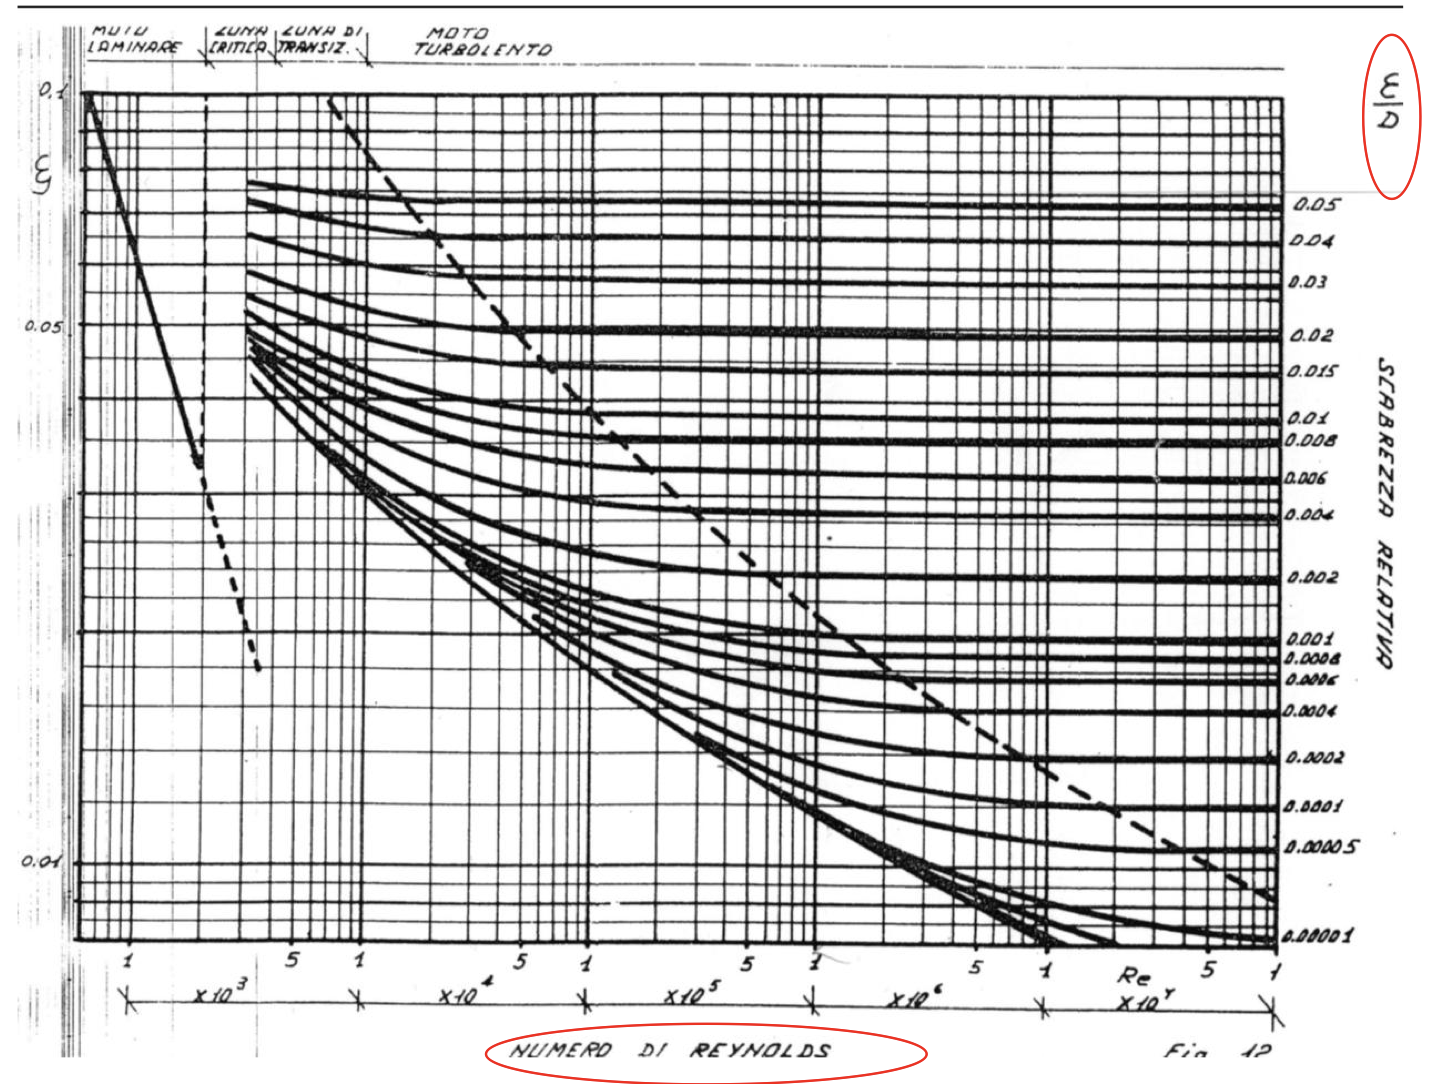
\includegraphics[width=0.9\linewidth]{assets/attrito.png}
    \caption{Calcolo del fattore di attrito}\label{fig:attrito}
\end{figure}

\begin{figure}
    \centering
    \begin{subfigure}{0.45\linewidth}
        \centering
        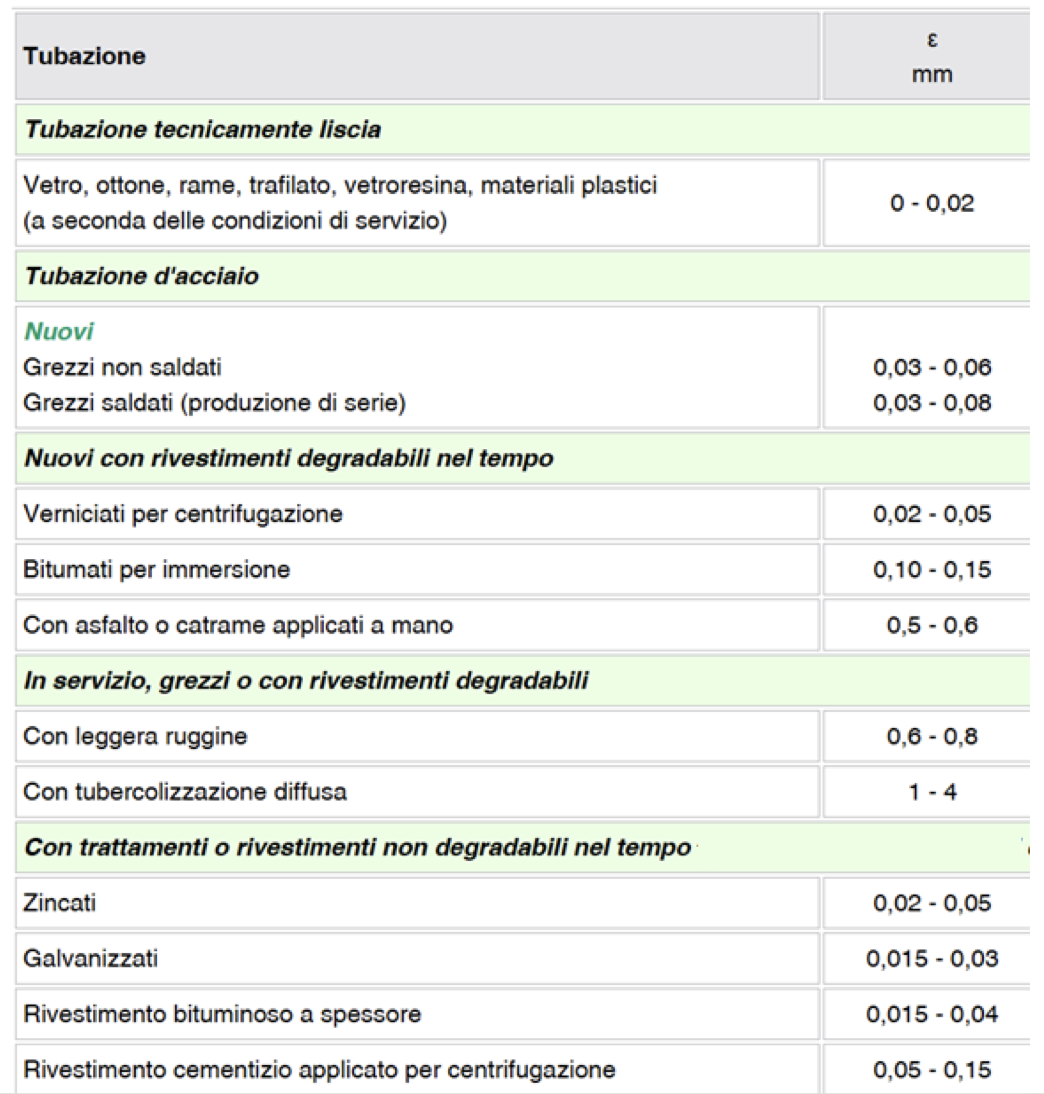
\includegraphics[width=\linewidth]{assets/scabrezza.png}
        \caption{Scabrezza}\label{fig:scabrezza}
    \end{subfigure}
    \begin{subfigure}{0.45\linewidth}
        \centering
        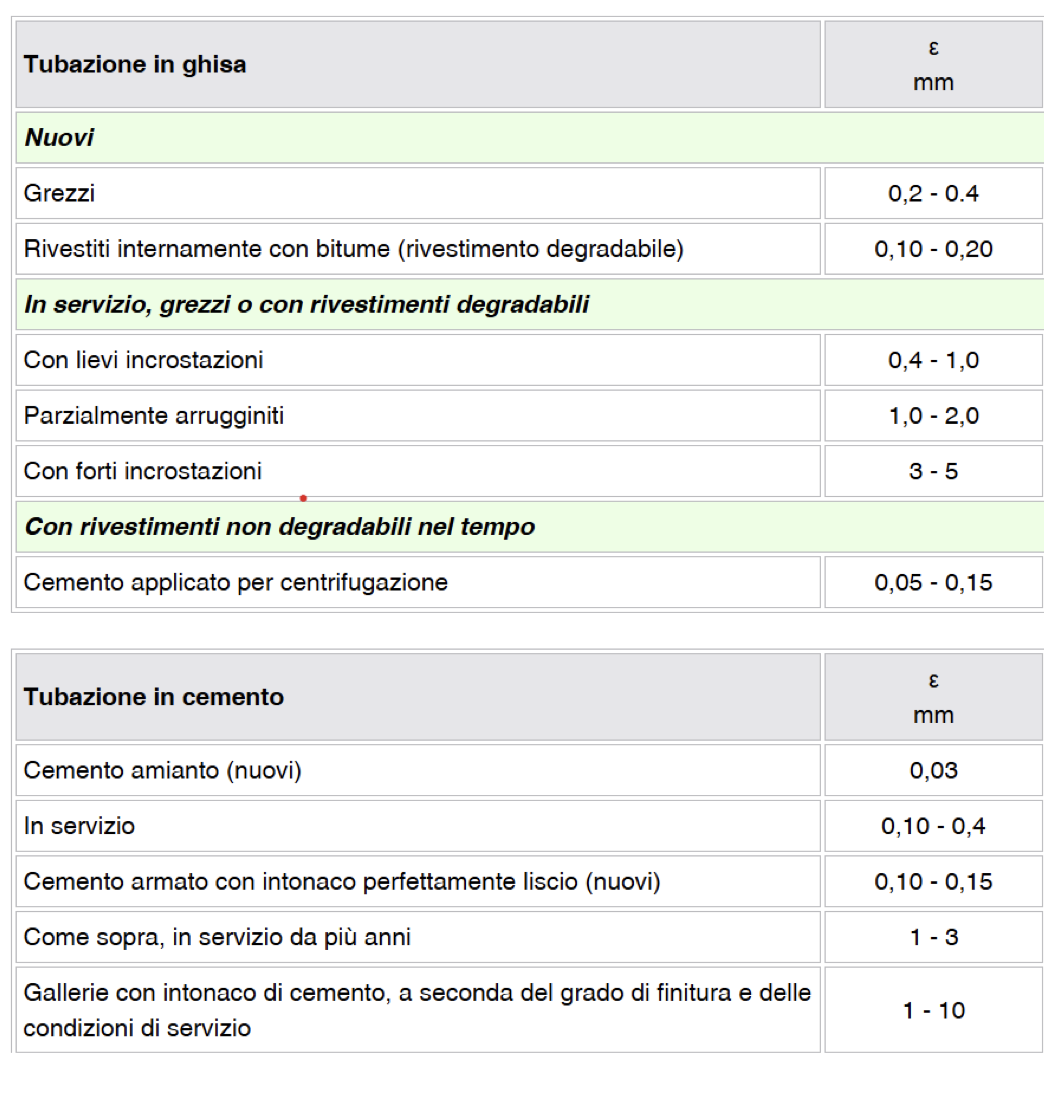
\includegraphics[width=\linewidth]{assets/scabrezzaghisa.png}
        \caption{Scabrezza ghisa}\label{fig:scabrezzaghisa}
    \end{subfigure}
\end{figure}

\begin{figure}
    \centering
    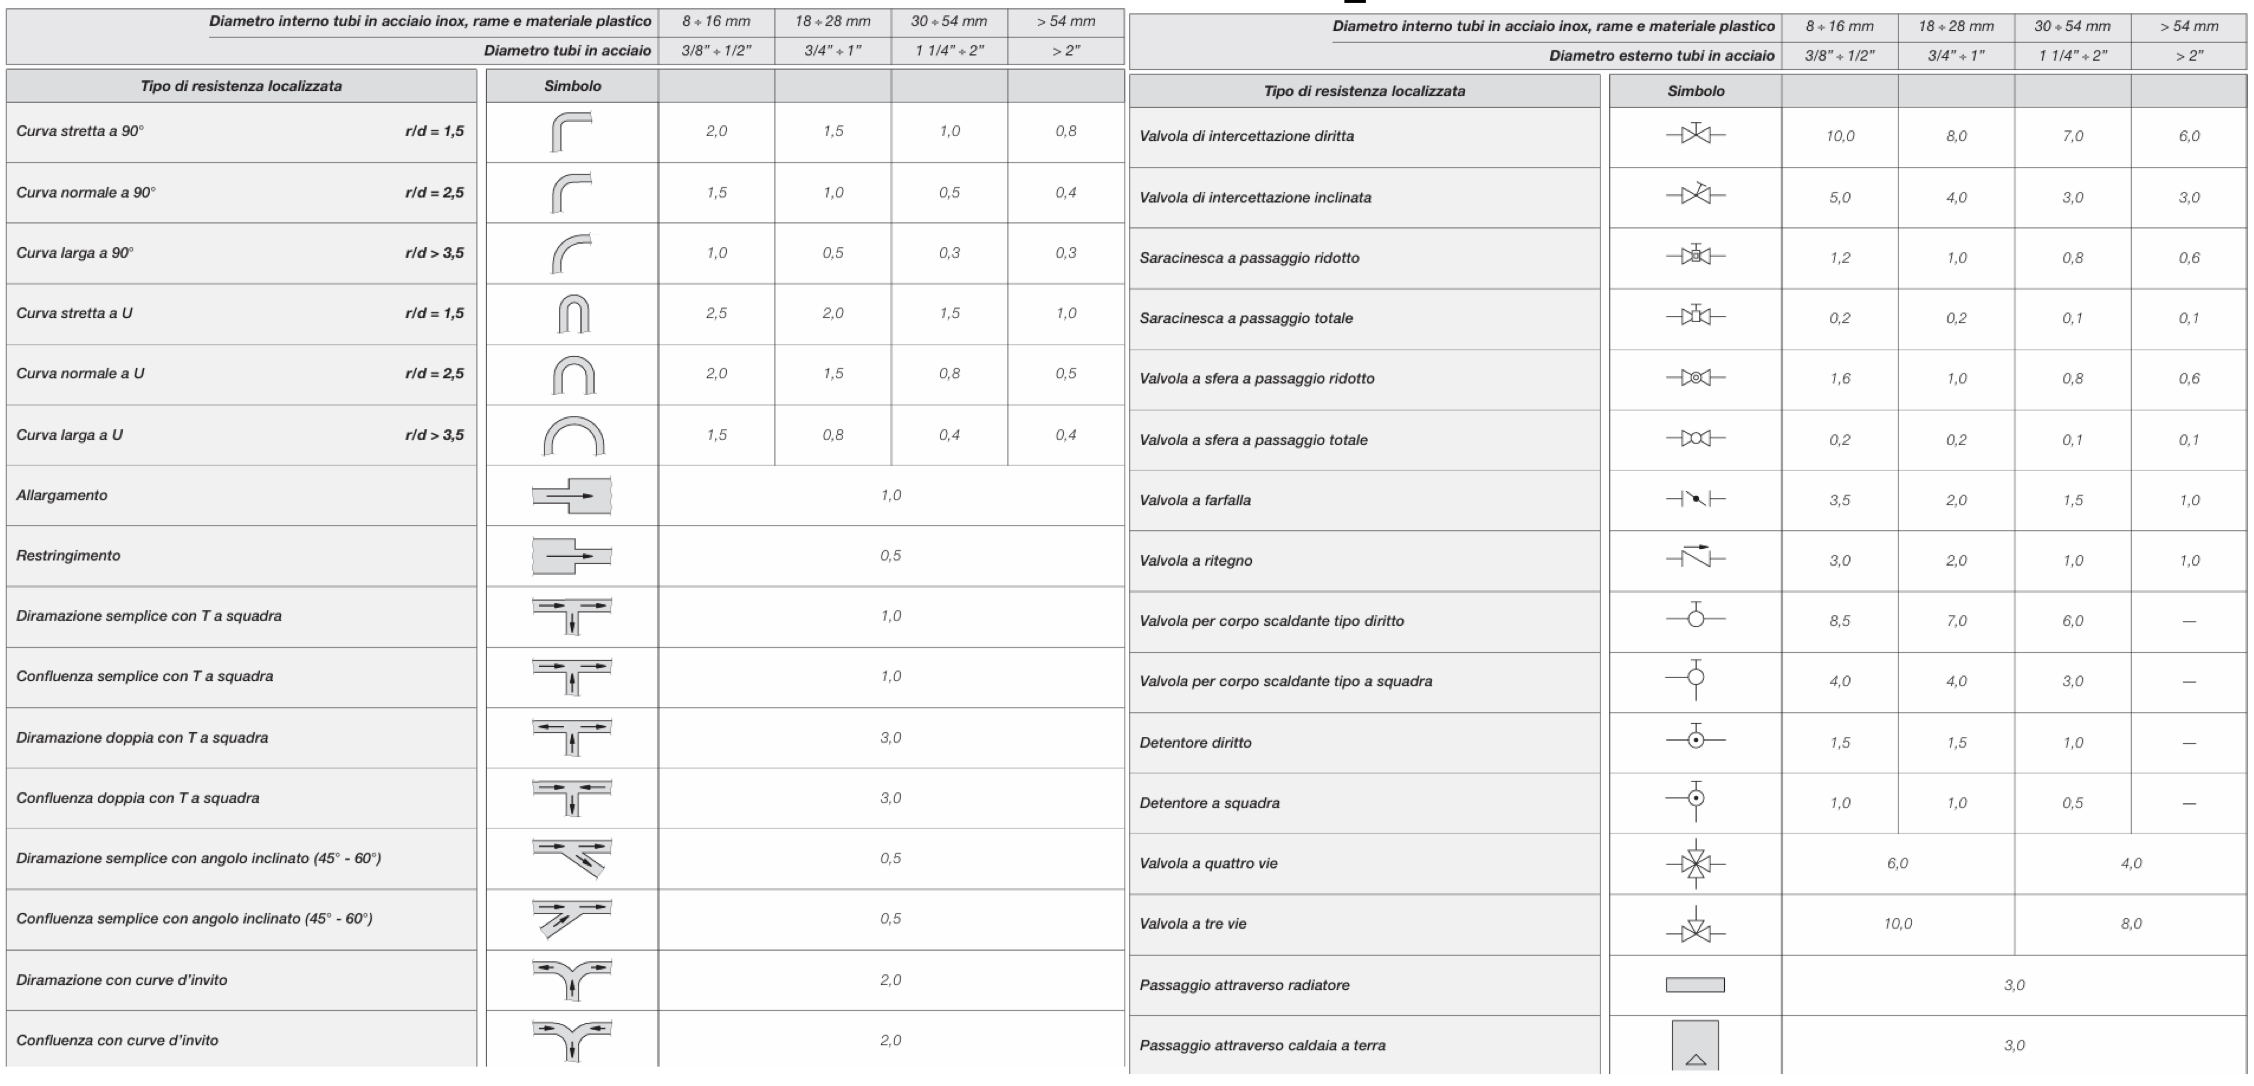
\includegraphics[width=0.9\linewidth]{assets/attritoconfentratoacqua.png}
    \caption{Attrito concentrato in acqua}\label{fig:attritoconfentratoacqua}
\end{figure}